%%%%%%%%%%%%%%%%%%%%%%%%%%%%%%%%%%%%%%%%%%
% Internship Report template
% Chemistry department 
% Version 1.1 (15/02/14)
%%%%%%%%%%%%%%%%%%%%%%%%%%%%%%%%%%%%%%%%%%

%----------------------------------------------------------------------------------------
%	PACKAGES AND OTHER DOCUMENT CONFIGURATIONS
%----------------------------------------------------------------------------------------

\documentclass[fleqn,10pt]{InternshipReport-ENS-PSL}

\setlength{\columnsep}{0.55cm} % Distance between the two columns of text
\setlength{\fboxrule}{0.75pt} % Width of the border around the abstract

\definecolor{color1}{RGB}{60,23,61} % Color of the article title and sections
\definecolor{color2}{RGB}{20,00,20} % Color of the boxes behind the abstract and headings


\usepackage{amsthm,amsmath,amssymb}
\usepackage{mathrsfs}
\usepackage{physics}
\usepackage{cancel} %用于在偏微分符号上画斜线
\usepackage{ulem} %波浪线, 双下划线
\usepackage{newcommand_yye}


%%%%% LOMA图标
%%左上角?右下角?
%\includegraphics[width=0.05\linewidth]{EmetBrownVF.png}


%%%%% 流程图用tikz
\usepackage{tikz}
\usetikzlibrary{positioning, shapes.geometric}
\usetikzlibrary{graphs, positioning, quotes, shapes.geometric}



%%%%% 页眉页脚
\pagestyle{fancy}
%\fancyhf{}
\fancyhead[RE,LO]{Yilin YE} % Right on Even page, Left on Odd page
%\fancyfoot[RE,LO]{NMR@ENS M1} % 每页左下角
%\fancyfoot[LE,RO]{Yilin YE} % 每页右下角
%\rhead{\includegraphics[width=0.8cm]{EmetBrownVF.png}} % 每页右上角,与页码冲突
%\lhead{\includegraphics[width=0.8cm]{Universitat_Bordeaux_Logo.png}}
\lfoot{
\includegraphics[height=0.7cm]{Universitat_Bordeaux_Logo.png} \includegraphics[height=0.6cm]{LOMA-CNRS-logo.png}
\includegraphics[height=0.8cm]{cnrs_logo.png}}
\rfoot{
\includegraphics[height=0.5cm]{anr_logo.png} \includegraphics[height=0.8cm]{erc_logo_1.png}
\includegraphics[height=0.8cm]{EmetBrownVF.png}}



%----------------------------------------------------------------------------------------
%	ARTICLE INFORMATION
%----------------------------------------------------------------------------------------

\ReportTitle{Brownian Motion near a Soft Surface} % Article title
\Author{Yilin YE}
\Supervisor{Yacine AMAROUCHENE, David DEAN, Thomas SALEZ}
\Laboratory{Université de Bordeaux, CNRS, Laboratoire Ondes et Matière d'Aquitaine, UMR 5798, F-33405, Talence, France}

\Keywords{Brownian motion --- soft surface --- Langevin equation --- noise correlator --- Fokker-Planck equation} 
\newcommand{\keywordname}{Keywords} 
% Defines the keywords heading name

%----------------------------------------------------------------------------------------
%	ABSTRACT
%----------------------------------------------------------------------------------------

\Abstract{
%\medskip
We consider the Brownian motion of a particle in 2D near a soft surface. We invoke previous deterministic soft-lubrication predictions for the forces and torques at leading order in compliance, and incorporate further thermal fluctuations in the description. Specifically here, a simple but model Winkler’s response is assumed for the soft substrate. \\

From the Fokker-Planck equation and the equilibrium constraint, we obtain the effective friction matrix as a function of the position variable and the geometric, viscous and elastic parameters. We also derive the proper noise correlators and spurious drifts to be used in the inertial Langevin equation. Solving numerically the latter requires a multi-dimensional discretisation. Our results demonstrate the influence of softness on various statistical observables.
}

%----------------------------------------------------------------------------------------

\begin{document}

\flushbottom % Makes all text pages the same height

\maketitle % Print the title and abstract box

\thispagestyle{empty} % Removes page numbering from the first page

%----------------------------------------------------------------------------------------
%	ARTICLE CONTENTS
%----------------------------------------------------------------------------------------


\section*{Introduction} % The \section*{} command stops section numbering
 


In 1827, Robert Brown, the British botanist, reported on the random motion of pollen particles under a microscope [ref]. The same thing happens with coal dust, leading to nothing about alive matters, which matched earlier observations [Jan Ingenhousz]. Brown speculated that the apparent random motion of colloids is a result of the thermal movement of surrounding solvent molecules, implying indirect evidences of atoms. %*** Echoes agnostic theory developed around that time by Dalton \& others, but there was no direct measurement or observation of atoms.
Other pioneers like Einstein and Perrin provided decisive evidence for the existence of atoms. 

In 1905, Albert Einstein proposed a stochastic model for Brownian motion [ref], indicating clean connection with the motion of impacts with atoms. With flux conservation, he recovered the microscopic diffusion equation $\pder[\rho]{t} = D \pdv[2]{\rho}{x}$, where $\rho$ is the probability density of particles as a function of time $t$ and displacement $x$, while $D$ refers to the diffusion coefficient, which describes the mobility of the particle inside a given liquid. 
At the same time, he also obtained $D = \frac{RT}{N_A \cdot 6\pi \eta r}$, where $\eta$ refers to viscocity, $r$ radius of particle, and $N_A$ Avogadro number. 
Specifically, free Brownian motion in the bulk could be characterized by a typical spatial extent evolving as the square root of time, as well as Gaussian displacements. Hence, one can measure the average displacement $\lambda$ after a delay $\tau$ as $\lambda = \sqrt{2D \tau}$. 

After Einstein's theoretical explanation, French physicist Jean Perrin did experiments and measured $N_A$ with different techniques, which confirmed Einstein's prediction, and the existence of atoms. For this great achievement, he was honored with the Nobel Prize for Physics in 1926. [ref]

The force required to move one particle in the fluid is proportional to its velocity, with friction coefficient $\zeta = 6 \pi \eta r$ shown by Stockes in 1850s. However, this result would lead to a zero velocity at long time limit, conflicting with the nature that particles would never stop. Based on that, Paul Langevin in 1908 furnished the formation in term of equations of motions and laws of mechanism. With a brillant idea, he introduced the concept of a random force or noise, toward the famous Langevin equation: [ref]
$$ m \dot{v} = - \zeta v + \dlt F $$
where the first term refers to systematic put of the environment influence, while the second term $\dlt F$ refers to the very sudden effect, random impacts due to thermal fluctuation with solvent molecules. Generally, there is no correlation in space and in time, so $\lla \dlt F(t) \rra = 0$. Also, Gaussian white noise would be exploited as $\lla \dlt F(\tau_1) \dlt F(\tau_2) \rra = 2 k_B T \zeta \dlt(\tau_1 - \tau_2)$, which could reflect well the fluctuation dissipation theorem [ref], Stokes-Einstein relation [ref], and Green-Kubo relations [ref].


Brownian motion has been a central paradigm in modern science, which presents numerous applications in physics [ref], biology [ref], and even finance for instance on share prices [ref?]. 
In addition, motility of microscopic biological matters towards certain targets is a paramount question of biophysics, such as: DNA replication, antibody recognition, and various self-assembly. Ideally, this problem could be simplified to mechanics through a basic combination of necessary ingredients: confined environment, elastic boundaries, thermal fluctuations, and viscous flow; %In echo to this point, a key problem of modern nanoscience amounts to understanding how to build the missing links between the antinomic molecular and continuum descriptions of matter or, stated differently, between the bottom-up and top-bottom approaches of condensed matter. 
as the soft contacts are ubiquitous in biology.


In soft matter, an emergent ElastoHydroDynamic (EHD) lift force was theoretically predicted recently [ref] for elastic bodies moving past each other in a fluid. 
This amazing effect has thus been explored with various deterministic models and experiments, showing its potential relevance for biological and nanoscale systems. 
For the sake of further understanding of EHD, the “EMetBrown” project was carried out with three core theoretical models: soft lubrication, stochastic theory and Langevin simulations. 
Indeed, several preliminary results have been published previously, containing EHD force measurement in 2020 \cite{PRL2020}, confined Brownian motion in 2021 \cite{PRR2021,MaxPhD}, rigid sphere near elastic wall in 2022 \cite{JFM2022}


To step further on physical description of biological motility by solving a fundamental problem at the boundary between continuum and statistical mechanics, there confronts challenges about Brownian motion near soft interfaces.
%The ambition of EMetBrown is to address this frontier challenge and set the ground for a new physical description of biological motility by solving a fundamental problem at the boundary between continuum and statistical mechanics: Brownian motion near soft interfaces. 
%There are three objectives revealed, explore and harvest the signatures of such motion, paving the way toward the design of new methods for the rheology of biological and nanoscale materials, surface patterning and medical research. 
%These objectives will be reached by a combination of experiments, theory and numerics – all of which are familiar to the PI from past research. 
% EMetBrown involves three core experimental setups (free colloids, optical trapping and atomic-force microscopy), three core theoretical models (soft lubrication, stochastic theory and Langevin simulations) and three exploratory tools (microfluidics, suspension rheometry and molecular dynamics). 
%These methods will be employed in four work packages, covering hard, soft, biological and fluctuating interfaces, as well as directive flow.
%The “EMetBrown” project thus naturally aims at filling this gap, and further utilizing the associated knowledge production towards applications as various and important as particle trapping and transport, surface patterning, non-contact rheology, or biological filtering. 
Exactly, the study of Brownian motion in soft-lubricated environments appears here as the canonical problems of biophysics and nanophysics. %Despite the obvious character of this statement, it is intriguing to notice that theoretical studies are scarce on the topic, and that experimental pieces of evidence are inexistant - to the best of our knowledge. 
However, it is still intriguing to note that studies are scarce on this topic. 
Therefore, a key mission arises, namely how to combine continuum ingredients, especially hydrodynamics and elasticity, together with molecular fluctuations at small scales. %The result is an original migration scenario at small scales – with enormous implications. 

In this internship report, we aim to develop theoretical framework on 3D non-linear EHD forces coupled by Langevin problem including multiplicative noise and external potential, then derive the effective friction and modified noise correlators. %In this context, and moving beyond the deterministic, the PI’s claim is that such EHD forces are even spontaneously triggered by thermal fluctuations. 
Besides, numerical simulations with multi-dimensional discretisation have also been completed to verify simultaneous experiments. The core strategy is to develop perturbation at leading order in compliance of soft surface, demonstrating the effect of softness on various statistical variables.





%------------------------------------------------

\section*{Theoretical Analyses}

\ssc*{Situation of the problem}

Herein, we consider a 2D particle's Brownian motion near a soft surface, based on the work in 2015 \cite{JFM2015}. Below are equations of motion, with three coupled variables: $X_G, \Dlt$ for parallel, vertical displacement, and $\Theta$ the rotation angle.

$$ \textcolor{red}{\ddot{X}_G} + \frac{2\varepsilon \xi}{3} \frac{\dot{X}_G}{\sqrt\Delta} + \frac{\textcolor{brown}{\kappa} \varepsilon \xi}{6} \left[ \frac{19}{4} \frac{\dot\Delta \dot{X}_G}{\Delta^{7/2}} - \frac{\dot\Delta \dot\Theta}{\Delta^{7/2}} + \frac{1}{2} \frac{\textcolor{blue}{\ddot{\Theta}} - \textcolor{red}{\ddot{X}_G}}{\Delta^{5/2}} \right] = 0 $$

$$ \textcolor{green}{\ddot{\Delta}} + \xi \frac{\dot{\Delta}}{\Delta^{3/2}} + \frac{\textcolor{brown}{\kappa} \xi}{4} \left[ 21 \frac{\dot{\Delta}^2}{\Delta^{9/2}} - \frac{(\dot\Theta - \dot{X}_G)^2}{\Delta^{7/2}} - \frac{15}{2} \frac{\textcolor{green}{\ddot{\Delta}}}{\Delta^{7/2}} \right] + \cos\alpha = 0  $$

$$ \textcolor{blue}{\ddot{\Theta}} + \frac{4\veps\xi}{3} \frac{\dot\Theta}{\sqrt\Delta} + \frac{\textcolor{brown}{\kappa} \veps \xi}{3} \left[ \frac{19}{4} \frac{\dot\Delta \dot\Theta}{\Delta^{7/2}} - \frac{\dot\Delta \dot{X}_G}{\Delta^{7/2}} + \frac{1}{2} \frac{\textcolor{red}{\ddot{X}_G} - \textcolor{blue}{\ddot{\Theta}}}{\Delta^{5/2}} \right] = 0  $$
\normalsize
where $\epsilon$ is the ratio of initial height and particle radius;
$\xi$ the ratio of free fall time and typical lubrication damping time;
$\kappa \ll 1$, dimensionless compliance for the soft wall deformation to describe elasticity.
In our case, we focus on a rigid support plan, so $\alpha=0$.

In these equations, the perpendicular height $\Dlt$ plays a significant role, leading to no possible analytical expressions for each variable. Also, velocities $\dot{X}_G, \dot{\Dlt}, \dot{\Theta}$ would interact with each other, at leading order of $\kpa$. Moreover, extra acceleration terms emerge with non-zero $\kpa$. Consider Brownian motion for such a system, we should describe the corresponding friction coefficient, and random force correlator as well. To simplify, we would address $r_x, r_z, r_\tta$ for three directions $X_G, \Dlt, \Theta$, and $v_x, v_z, v_\tta$ for $\dot{X}_G, \dot{\Dlt}, \dot{\Theta}$.

\begin{figure}[ht]
\centering
\includegraphics[width=0.9\linewidth]{BEHDfig_YYE.pdf}
\caption{Schematic of the system. A negatively buoyant cylinder (grey) falls down under the influence of gravity $\mathbf{g}$, inside a viscous fluid (blue), in the vicinity of a thin soft wall (yellow). The ensemble lies atop a infinitely rigid support (black).}
\label{fig-onecol}
\end{figure}


Herein, we would first start from Langevin equation for explicit expressions of velocities $v(t)$. By computing the time average of velocity square $\lla v^2(t) \rra$ , we could figure out the noise correlator amplitudes $\lla \dlt F(\tau_1) \dlt F(\tau_2) \rra$. Also, by $\lla v(0) v(t) \rra$ we could derive the mean square displacement (MSD) $\lla \Dlt r^2 \rra$ and the diffusion coefficients as well.
\begin{center}
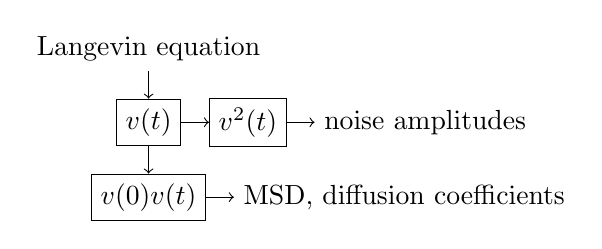
\begin{tikzpicture}[node distance=10pt]
  \node[, rounded corners]                        (LE)   {Langevin equation};
  \node[draw, below=of LE]                         (vt)  {$v(t)$};
  \node[draw, right=of vt]                        (vtsq)  {$\lla v^2(t) \rra $};
  \node[draw, below=of vt] (v0vt) {$\lla v(0) v(t) \rra $};
  \node[, right=of vtsq] (famp) {noise amplitudes};
  %\node[draw, right=of v0vt] (msd) {$\lla \Delta r^2 (t) \rra$};
  \node[, right=of v0vt] (MSD) {MSD, diffusion coefficients};
  %\node[, below=of MSD] (diff) {diffusion coefficient};
  
  \draw[->] (LE)  -- (vt);
  \draw[->] (vt) -- (vtsq);
  \draw[->] (vt) -- (v0vt);
  \draw[->] (vtsq) -- (famp);
  %\draw[->] (v0vt) -- (msd)
  %\draw[->] (v0vt) -- (diff);
  \draw[->] (v0vt) -- (MSD);
\end{tikzpicture}
\end{center}


\ssc*{Effective friction matrix}
In Langevin equation, the parameter $\gma$ plays a paramount role to reflect the friction property of a given environment. This parameter would result in several important variables mentioned above. Therefore, in this subsection, we would derive effective friction matrix according to equations of motion, considering parameters before velocities as friction and those before accelerations as the effective mass.

\begin{center}
\begin{tikzpicture}[node distance=10pt]
  \node[draw] (coefm) {$\dot{v}_i$ coefficients};
  \node[draw, below=of coefm] (grandm) {mass matrix $M_{\ab} (\textcolor{brown}{\kappa})$};
  \node[draw, below=of grandm] (morg) {real mass $m_i$};
  \node[draw, below=of morg] (gmaorg) {friction matrix $\gma_{\ab} (\textcolor{brown}{\kappa})$};
  \node[draw, below=of gmaorg] (coefv) {$v_i$ coefficients};
  \node[draw, right=30pt of morg] (gmaeff) {effective friction $\gamma_{\mathrm{eff}} (\textcolor{brown}{\kappa})$}  
  
  \draw[->] (coefm)  -- (grandm);
  \draw[->] (coefv) -- (gmaorg);
  \draw[->] (grandm) -- (gmaeff);
  \draw[->] (gmaorg) -- (gmaeff);
  \draw[->] (morg) -- (gmaeff);
\end{tikzpicture}
\end{center}


\sss*{Mass matrix}
Consider the deterministic equation with Einstein summation convention on $\bt$:
$$ m_\al \cdot \dot{v}_\al = \left[ F_{1\al}(\bbf{x}) + F_{2\ab}(\bbf{x}) \dot{v}_\bt \right] - m_\al \cdot \gamma_{\ab} v_\bt $$
where $\bbf{x}$ is the position vector, $F_{1\al}(\bbf{x})$ refers to forces only depending on positions like external potentials, $F_{2\ab}(\bbf{x})$ are coefficients for accelerations, and $\gamma_{\ab}$ those before velocities. For $z,x$ components, the mass $m_\alpha = m = \pi r^2 \rho$, namely the mass of the column (per unit length); while $m_\theta = mr^2 /2$ refers to the moment of inertia. 

Introduce the mass matrix as $M_{\alpha\beta} = \delta_{\alpha\beta} \cdot m_\alpha - F_{2h\alpha\beta}(\bbf{x})$.
%According to equations of motion mentioned before, we divide EHD interactions into two parts: \\
We extract easily all non-zero $F_{2h\alpha\beta}(\bbf{x})$ according to extra acceleration terms: %Along the perpendicular direction, 
$$ \agn{
F_{2hzz} = - \frac{m_z a_5}{\Delta^{7/2}} \fives& F_{2hxx} = - \frac{m_x b_5}{\Delta^{5/2}} \fives F_{2hx\tta} = - \frac{m_x b_4}{\Delta^{5/2}} \\
\fives& F_{2h\tta x} = - \frac{m_\tta c_4}{\Delta^{5/2}} \fives F_{2h\tta\tta} = - \frac{m_\tta c_5}{\Delta^{5/2}}
} $$
where $a_5 = -\frac{15\kappa\xi}{8}$, $b_4 = - b_5 = \frac{\kappa\xi\veps}{12}$, $c_4 = - c_5 = \frac{\kappa\xi\veps}{6}$. As a result, we have the mass matrix $M$
$$ M = \left(
\begin{array}{ccc}
 m_z-\frac{15 \kappa  \xi  m_z}{8 \Delta ^{5/2}} & 0 & 0 \\
 0 & m_x -\frac{\kappa  \xi  \epsilon  m_x}{12 \Delta ^{5/2}} & \frac{\kappa  \xi  \epsilon  m_x}{12 \Delta ^{5/2}} \\
 0 & \frac{\kappa  \xi  \epsilon  m_{\theta }}{6 \Delta ^{5/2}} & m_{\theta }-\frac{\kappa  \xi  \epsilon  m_{\theta }}{6 \Delta ^{5/2}} 
\end{array} \right) $$
and its inverse matrix at first-order approximation of $\kappa$:
$$ M^{-1} \approx \left(
\begin{array}{ccc}
 \frac{1}{m_z}+\frac{15 \kappa  \xi }{8 \Delta ^{5/2} m_z} & 0 & 0 \\
 0 & \frac{1}{m_x}+\frac{\kappa  \xi  \epsilon }{12 \Delta ^{5/2} m_x} & -\frac{\kappa \xi  \epsilon}{12 \Delta ^{5/2} m_{\theta }} \\
 0 & -\frac{\kappa \xi  \epsilon}{6 \Delta ^{5/2} m_x} & \frac{1}{m_{\theta }}+\frac{\kappa  \xi  \epsilon }{6 \Delta ^{5/2} m_{\theta }} 
\end{array}
\right) $$


\sss*{Fokker-Planck equation for friction matrix}
Consider the following deterministic equation
$ d \bbf{x} = \bbf{v} dt $
and $ d \bbf{v} = - \bbf{U} dt - \bbf{\nabla} \phi(\mathbf{x}) dt $.
We assume that $\bbf{U}$ are generated by hydrodynamic interactions, which do not however affect the equilibrium Gibbs-Boltzmann distribution which is 
$$ P_{eq} (\mathbf{x},\mathbf{v}) = \frac{1}{\bar{Z}} \exp \left( - \frac{\beta \mathbf{v}^2}{2} - \beta \phi(\mathbf{x}) \right) $$
where $\beta^{-1} = k_B T$. Note $\pder[P]{x_\alpha} = P \left( -\beta \pder[\phi]{x_\alpha} \right)$, $\pder[P]{v_\alpha} = P \left( -\beta v_\alpha \right)$. To follow the evolution of the distribution probability $P(\bbf{x},t)$, we exploit the Fokker-Planck equation, solving % with the operator $H_{FP}$
$$ \pder[P]{t} = \pder{v_\alpha} \left[ T \gamma_{\alpha\beta} \pder[P]{v_\beta} + U_\alpha P + \pder[\phi]{x_\alpha} P \right] - \pder{x_\alpha} v_\alpha P $$
The last two terms would vanish, %since
%$$ \pder{v_\alpha} \left( \pder[\phi]{x_\alpha} P \right) = \cancel{ \left( \pder{v_\alpha} \pder[\phi]{x_\alpha} \right) } \cdot P + \pder[\phi]{x_\alpha} \cdot \pder[P]{v_\alpha} = \pder[\phi]{x_\alpha} \cdot P (-\beta v_\alpha) $$
%$$ \pder{x_\alpha} \llp v_\alpha P \rrp = \cancel{ \left( \pder[v_\alpha]{x_\alpha} \right) } P + v_\alpha \left( \pder[P]{x_\alpha} \right) = v_\alpha \cdot P \cdot \left( -\beta \pder[\phi]{x_\alpha} \right) $$
so we have
$$ \pder[P]{t} = \pder{v_\alpha} \left[ T \gamma_{\alpha\beta} \pder[P]{v_\beta} + U_\alpha P \right] = \pder{v_\alpha} \left[ - \gamma_{\alpha\beta} v_\beta P + U_\alpha P \right] $$
Therefore, at equilibrium $\pder[P]{t} = 0$, we obtain the GB distribution for the steady state if 
$$ U_\alpha = \gamma_{\alpha\beta} v_\beta $$



Following the format of Langevin equation, $\gamma_{\ab}$ matrix above only contains terms about first derivatives %does not contain coefficients $(a/b/c)_{5/6}$
$$ \agn{
\gamma_{Z\beta} v_\beta &= a_1 \frac{\dot{\Delta}}{\Delta^{3/2}} + a_2 \frac{\dot{\Delta}^2}{\Delta^{9/2}} + a_3 \frac{\dot\Theta^2 + \dot{X}^2}{\Delta^{7/2}} + a_4 \frac{\dot\Theta \dot{X}}{\Delta^{7/2}}\\
\gamma_{X\beta} v_\beta &= b_1 \frac{\dot{X}}{\sqrt\Delta} + b_2  \frac{\dot\Delta \dot{X}}{\Delta^{7/2}} + b_3 \frac{\dot\Delta \dot\Theta}{\Delta^{7/2}} \\
\gamma_{\Theta\beta} v_\beta &= c_1 \frac{\dot\Theta}{\sqrt\Delta} + c_2 \frac{\dot\Delta \dot\Theta}{\Delta^{7/2}} + c_3 \frac{\dot\Delta \dot{X}}{\Delta^{7/2}} 
} $$
with reduced parameters like $a_1 = \xi$, $b_1 = \frac{2 \veps \xi}{3}$, and so on for convenience. %\{Based on the equilibrium hypothesis from Fokker-Planck equation  (\textit{need details?}) ...\} 
To be general, we write $\gma$ for small velocities as
$$ \gamma_{\alpha\beta} v_\beta = \lambda_{\alpha\beta}(\mathbf{x}) v_\beta + \Lambda_{\alpha\beta\gamma} (\mathbf{x}) v_\beta v_\gamma $$ 
where the term $\lambda_{\alpha\beta}(\mathbf{x})$ is just the friction tensor without any elastic effects. Additional efforts should be taken on the second term by symmetry. We would like to have 
$$ \gamma_{\alpha\beta} = \lambda_{\alpha\beta} + \gamma_{2\alpha\beta} \tens \gamma_{2\alpha\beta} = \Gamma_{\alpha\beta\gamma} v_\gamma $$
Consequently, we have 
$ \Gamma_{\alpha\beta\gamma} (\mathbf{x}) v_\beta v_\gamma = \Lambda_{\alpha\beta\gamma} (\mathbf{x}) v_\beta v_\gamma $. 
Without loss of generality, we take $\Lambda_{\alpha\beta\gamma} = \Lambda_{\alpha\gamma\beta}$, which then gives $\Gamma_{\alpha\beta\gamma} + \Gamma_{\alpha\gamma\beta} = 2 \Lambda_{\alpha\beta\gamma}$. In fact, velocity terms on different directions contribute equally for products, so $\Lambda_{\alpha\beta\gamma} = \Lambda_{\alpha\gamma\beta}$. Also, mutual interactions means that terms with $v_\al$ contribute equally toward $\gma_{\ab} v_\bt$, hence we obtain another constraint $\Gamma_{\alpha\beta\gamma} = \Gamma_{\beta\alpha\gamma}$. Combine those conditions together, we get $\gma_{\ab}$ at leading-order of $\kpa$:
$$ \agn{
\gamma_{zz} &\approx  \frac{\xi}{\Delta ^{3/2}} + \frac{21 \kxi v_z}{4 \Delta^{9/2}} \\
\gamma_{xx} &\approx  \frac{2 \epsilon \xi}{3 \sqrt{\Delta}} +\frac{(6 + 19 \epsilon ) \kxi v_z}{24 \Delta^{7/2}} \\
\gamma_{\theta\theta} &\approx  \frac{4 \epsilon \xi}{3 \sqrt{\Delta}} + \frac{(3 + 19 \epsilon ) \kxi v_z}{12 \Delta^{7/2}} 
} $$

$$ \agn{
\gamma_{zx} = \gamma_{xz} &\approx \frac{\kappa  \xi  \left(( 3 + \epsilon) v_{\theta } - 3 v_x \right)}{12 \Delta ^{7/2}} \\
\gamma_{z\theta} = \gamma_{\theta z} &\approx \frac{\kappa  \xi  \left((3 - \epsilon) v_x - 3 v_{\theta } \right)}{12 \Delta ^{7/2}}\\
\gamma_{x\theta} = \gamma_{\theta x} &\approx -\frac{\kappa  \xi  (\epsilon +1) v_z}{4 \Delta ^{7/2}}
} $$

The Langevin equation corresponding to this is, using the Itô convention,
$$ \dv[]{v_\alpha}{t} = - U_\al - \pder[\phi]{x_\al} + k_B T \pder[\gma_{\ab}]{v_\bt} + \dlt F_\al $$
which can be written as
$$ \dv[]{v_\alpha}{t} = - U_\al - \pder[\phi]{x_\al} + k_B T \Gamma_{\al\bt\bt} + \dlt F_\al $$
Note, we only have non-zero $\Gamma_{\al\bt\bt}$ 




\sss*{Effective friction matrix}
Therefore, the deterministic equation turns to \\
$ m_{\al} \cdot \dot{v}_\al &- F_{2\ab}(\bbf{x}) \dot{v}_\bt = M_{\ab} \dot{v}_\beta = F_{1\al}(\bbf{x}) - m_\al \cdot \gamma_{\ab} v_\beta $ \\
and then we could finally find the effective friction matrix as $\gamma_\mrm{eff} =  M_{\ab}^{-1} m_\al \cdot \gma_{\ab} v_\bt$ % $$ \dot{v}_\bt &= M_{\ab}^{-1} \left( F_{1\al}(\bbf{x}) - m_\al \cdot \gamma_{\ab} v_\beta \right) $$
% $$ \gamma_\mrm{eff} = M_{\ab}^{-1} \cdot \left(\begin{array}{ccc}m_Z & 0 & 0 \\0 & m_X & 0 \\0 & 0 & m_\Theta \end{array}\right) \cdot \gamma_{\ab} $$
with elements below:
$$ \agn{
\gamma_{\mrm{eff},zz} &\approx \frac{\xi }{\Delta ^{3/2}} +\kappa  \left(\frac{15 \xi ^2}{8 \Delta^4}+\frac{21 \xi v_z}{4 \Delta ^{9/2}}\right) \\ % rang 1
\gamma_{\mrm{eff},xx} &\approx \frac{2 \xi  \epsilon }{3 \sqrt{\Delta }}+\frac{\kappa  \xi  \left(4 \sqrt{\Delta } \xi  \epsilon^2 + 18 v_z + 57 \epsilon  v_z \right)}{72 \Delta ^{7/2}} \\ % rang 2
\gamma_{\mrm{eff},\theta\theta} &\approx \frac{4 \xi  \epsilon }{3 \sqrt{\Delta }}+\frac{\kappa  \xi  \left(8 \sqrt{\Delta } \xi  \epsilon ^2+57 \epsilon  v_z+9 v_z\right)}{36 \Delta ^{7/2}} \\ % rang 3
\gamma_{\mrm{eff},xz} &= \gamma_{\mrm{eff},zx} \approx \frac{\kappa  \xi  \left((\epsilon +3) v_{\theta }-3 v_x \right)}{12 \Delta ^{7/2}}  \\ % rang 4
\gamma_{\mrm{eff},\theta z} &= \gamma_{\mrm{eff},z\theta} \approx \frac{\kappa \xi  \left( (3 -\epsilon) v_x - 3 v_{\theta } \right)}{12 \Delta ^{7/2}} \\ % rang 5
\gamma_{\mrm{eff},\theta x} &= \gamma_{\mrm{eff},x\theta} \approx -\frac{\kappa \xi  \left(16 \Delta ^3 \xi  \epsilon ^2+36 \Delta ^{5/2} (\epsilon +1) v_z\right)}{144 \Delta ^6} % rang 6
} $$







\ssc*{Modified noise correlator amplitude} %\label{corr}
After the effective friction matrix $\gamma_\rm{eff}$, we consider the random forces and their correlator amplitudes. For the 1D case in the bulk, we only need the square root of friction coefficient. Similarly, we could suppose that $\gamma_{\mrm{eff}} \approx \Psi + \kappa \Phi$, %where $\Psi$ is zero-order matrix of $\kpa $, while $\Phi $ the first-order one.
%$\Psi_i = \mrm{SeriesCoefficients} [\mrm{Series}[\gma_{\mrm{eff},ii},\{\kpa,0,0\} ], 0]$ \\
%$\Phi_i = \mrm{SeriesCoefficients} [\mrm{Series}[\gma_{\mrm{eff},ij},\{\kpa,0,1\} ], 1]$ \\
as well as $\gamma^{1/2}_\mrm{eff} \approx \psi + \kpa\chi$, then we have
$$ \gamma_{\mrm{eff}} = \gamma_{\mrm{eff}}^{1/2}\gamma_{\mrm{eff}}^{1/2} = (\psi + \kappa\chi)(\psi + \kappa\chi) \approx \psi\psi + \kappa (\psi\chi + \chi\psi) $$
so we resolve \(\psi_{ij} =\sqrt{\Psi_{ij} }\), and $\chi_{ij} = \frac{\Phi_{ij}}{\sqrt{\Psi_{ii}} + \sqrt{\Psi_{jj}}}$. Even though mass matrix should be taken into account later, we could always continue the same procedure.

%Consider the case without unit mass, we have to calculate the inverse mass matrix as an analogy of $\frac{1}{m}$, hences $\gamma_{\mrm{eff}}^{1/2} \to \llp \gamma_{\mrm{eff}} \cdot M^{-1} \rrp^{1/2}$ as an asymmetric matrix. Even though we could neglect the non-diagonal elements as the cross-correlated noise since $\kpa \ll 1$, we are still motivated to clarify these terms by proper treatment, such as the diagonalisation. However, we could hardly furnish a simple diagonalized matrix, numerical method would be expected. After extracting noise eigenvalues, we exploit the inverse base transform to furnish the exact contribution on each direction. Further discussion see subsection \ref{Discretisation algorithm}.


The results seem plausible and enough with the first-order correction of $\kappa$. However, as for $\gamma_\rm{eff}$, several velocities have been included. In 1D case, we make Laplace and the its inverse transform for solutions, while here we have to consider that as a matrix equation
%$$ \dot{\bbf{v}}_{3\times1} = - \gamma_{\rm{eff},3\times3} \cdot \bbf{v}_{3\times1} + M^{-1}_{3\times3} \cdot \delta F_{3\times1} $$
%and consider the corresponding Laplace transform
$$ \widetilde{\dot{\bbf{v}}} = - \widetilde{\gamma_{\rm{eff}} \cdot \bbf{v}} + \widetilde{M^{-1} \cdot \bbf{\delta F}} $$
Note, $\gamma_{\mrm{eff}}$ is not a constant matrix, which should be included inside the Laplace transform.
%We could not extract this friction matrix outside the Laplace transform, while similar for $M^{-1}$. 
%We try the Laplace transform directly on $-\widetilde{\gamma_{\rm{eff}} \cdot \bbf{v}}$, obtaining

%The Laplace transform of multiplication would be quite complex, since 
%$$ \widetilde{f(t)g(t)}(p) = \frac{1}{2\pi i} \lim_{T \to \infty} \int_{c-iT}^{c+iT} \widetilde{f}(s) \widetilde{g}(p-s) ds $$ 
%The integration is done along the vertical line $\Re(s)=c$ that lies entirely within the region of convergence of $\widetilde{f}$. For example, $f(t) = e^t$ does not possess a convergent Laplace integral if $\Re p>1$ or if $\Re p<1$. The strip of convergence has contracted to a line: the integral converges only where $\Re p=1$, and even then not exactly at $p=1$. We'd like to consider this part after getting the proper formula of $v_i$. For instance, if $f(t) = e^{-\gamma t}$ with $t>0$, we have the convergence strip if $\Re p > - \gamma$, which could be satisfied in our issue if we have a constant $\gamma$.


Dissect $\gamma_\rm{eff}$ as $\gamma_{\rm{eff}} = \gamma_{0} + \gamma_{1}(\kpa) + \gamma_{1v}(\kpa,v_i)$, 
$$ \gamma_0 = \left(\begin{array}{ccc} \frac{\xi }{\Delta ^{3/2}} & 0 & 0 \\0 & \frac{2 \xi  \epsilon }{3 \sqrt{\Delta }} & 0 \\0 & 0 & \frac{4\xi \eps}{3\sqrt{\Delta}}  \end{array}\right) $$
$$ \gamma_1 = \left(\begin{array}{ccc} \frac{15 \kappa \xi ^2}{8 \Delta ^4} & 0 & 0 \\0 &  \frac{ \kappa  \xi^2  \epsilon ^2}{18 \Delta^3} & -\frac{\kappa \xi^2 \eps^2}{9 \Delta^3} \\0 & -\frac{\kappa \xi^2 \eps^2}{9 \Delta^3} &  \frac{2 \kappa \xi^2 \eps^2}{9 \Delta^3} \end{array}\right) $$
$$ \gamma_{1v} = \left(\begin{array}{ccc} \frac{21 \kappa\xi v_z}{4 \Delta ^{9/2}} & \frac{\kxi  \left((\epsilon +3) v_{\theta }-3 v_x\right)}{12 \Delta ^{7/2}} & \frac{\kxi  \left( (3 - \epsilon) v_x - 3 v_{\theta} \right)}{12 \Delta ^{7/2}} \\ \frac{\kxi  \left((\epsilon +3) v_{\theta }-3 v_x\right)}{12 \Delta ^{7/2}} & \frac{\kappa\xi (6 + 19 \eps) v_z}{24 \Delta^{7/2}} & - \frac{\kappa \xi (\eps+1) v_z}{4 \sqrt{\Delta}} \\ \frac{\kxi  \left( (3 - \epsilon) v_x - 3 v_{\theta} \right)}{12 \Delta ^{7/2}} & - \frac{\kappa \xi (\eps+1) v_z}{4 \sqrt{\Delta}} & \frac{\kappa\xi (19 \eps + 3) v_z}{12 \Delta^{7/2}} \end{array}\right) $$
where $\gamma_0$ is constant matrix, independent on $\kpa$; $\gma_1$ depends on $\kpa$; and $\gamma_{1v}$ depends on $\kpa$ and velocities $v_i$. 
Hence we could separate the transform as $\widetilde{\gamma_{\rm{eff}} \cdot \bbf{v}} = \gamma_0 \cdot \widetilde{\bbf{v}} + \gamma_1 \cdot \widetilde{\bbf{v}} + \widetilde{\gamma_{1v} \cdot \bbf{v}}$. Since $\gma_0$ is a diagonal matrix, we write $\gma_{i0} = \gma_{i0}$ for the convenience. Also, we suppose that $\gamma_{1v,ij} = g_{ij\alpha} v_\alpha$, where $g_{ij\alpha}$ refers to the coefficient of $v_\alpha$ in $\gamma_{1v,ij}$, such as $g_{12x} = -\frac{\kxi v_x}{4 \Delta^{7/2}}$. A symmetric $\gamma_{\rm{eff}}$ results in symmetric $\gamma_0$ and $\gamma_1$, so is $g_{ij\alpha}$. 

It would be raisonnable to consider the perturbation on $\kpa$, for this elastic compliance parameter $\kappa \ll 1$ (about $10^{-4} \sim 10^{-3}$). We write $\bbf{v} = \bbf{v}_0 + \bbf{v}_1$, where the former is on 0 order while the latter 1 order. Similarly, the mass matrix and random forces would be treated in the same way.
$$ \agn{ \dot{\bbf{v}} &= \dot{\bbf{v}}_0 + \dot{\bbf{v}}_1 = - \gma_{\mrm{eff}} \cdot \bbf{v} + M^{-1} \cdot \bbf{\dlt F} \\ % rang 1
&= - (\gma_0 + \gma_1 + \gma_{1v}) \cdot (\bbf{v}_0 + \bbf{v}_1) + (M^{-1}_0 + M^{-1}_1) \cdot (\bbf{\dlt F}_0 + \bbf{\dlt F}_1 ) }$$
We only keep terms of 0 and 1 order of $\kpa$:
$$ \dot{\bbf{v}}_0 = - \gma_0 \cdot \bbf{v}_0 + M^{-1}_0 \cdot \bbf{\dlt F}_0 $$
$$ \dot{\bbf{v}}_1 = - \gma_0 \cdot \bbf{v}_1 - \gma_1 \cdot \bbf{v}_0 - \gma_{1v} \cdot \bbf{v}_0 + M^{-1}_0 \cdot \bbf{\dlt F}_1 + M^{-1}_1 \cdot \bbf{\dlt F}_0 $$
After Laplace transform, we have
$$ s \widetilde{\dot{\bbf{v}}}_0 - \bbf{v}(0) = - \gma_0 \cdot \wtd{\bbf{v}}_0 + M^{-1}_0 \cdot \wtd{\bbf{\dlt F}_0} $$
$$ s \widetilde{\dot{\bbf{v}}}_1 = - \gma_0 \cdot \wtd{\bbf{v}}_1 - \gma_1 \cdot \wtd{\bbf{v}}_0 - \wtd{\gma_{1v} \cdot \bbf{v}_0} + M^{-1}_0 \cdot \wtd{\bbf{\dlt F}_1} + M^{-1}_1 \cdot \wtd{\bbf{\dlt F}_0} $$
Note $\mathcal{L}_t\left[\int_0^t f(\tau ) g(t-\tau ) \, d\tau \right](s) = \left(\mathcal{L}_t[f(t)](s)\right) \left(\mathcal{L}_t[g(t)](s)\right)$. 0-order solutions are rather simple:
$$ v_{i0}(t) = v_{i0}(0) e^{-\gma_{i0} t} + \int_0^t \mrm{d}\tau \frac{\delta F_{i0} (\tau)}{m_i} \exp\left[-\gma_{i0}(t-\tau)\right] $$
Follow the same process we have done previously, we get the amplitude of noise correlator:
$$ \llang \delta F_{i0} (\tau_1) \delta F_{j0} (\tau_2) \rrang = 2 k_B T m_i \gamma_{i0} \delta_{ij} \delta(\tau_1 - \tau_2) $$

As for the 1-order correction $v_{i1}$, we have
$$ \agn{ (s + \gma_{i0}) \wtd{v_{i1}} &= - \sum_j \gma_{1,ij} \wtd{v_{i0}} - \sum_j \sum_k g_{ijk}  (\wtd{v_{j0} \cdot v_{k0}}) \\
& \fives + M^{-1}_{0i} \wtd{\dlt F_{i1}} + \sum_j M^{-1}_{1,ij} \wtd{\dlt F_{j0}} } $$
Laplace and its inverse transform have been calculated. To be clear, we decompose $\bbf{v}_1$ as
$$ \bbf{v}_{1} = \bbf{v}_{gv} + \llp \bbf{v}_{vv} + \bbf{v}_{vf} + \bbf{v}_{fv} + \bbf{v}_{ff} \rrp + \bbf{v}_{fm} + \bbf{v}_{mf} $$
with the following expressions along the direction $i$:
\normalsize
$$  v_{i,gv} = \frac{\gma_{1,ij}}{\gma_{i0} - \gma_{j0}} \lls \llp e^{- \gma_{i0} t} - e^{-\gma_{j0} t} \rrp v_j (0) + \int_0^t \mrm{d}\tau \frac{\dlt F_{j0}(\tau)}{m_j} \lls e^{- \gma_{i0} (t-\tau)} - e^{-\gma_{j0} (t-\tau)} \rrs \rrs $$
$$ v_{i,vv} = - g_{ijk} v_j (0) v_k (0) \cdot \frac{e^{-(\gma_{j0} + \gma_{k0}) t} - e^{-\gma_{i0} t}}{\gma_{i0} - \gma_{j0} - \gma_{k0}} $$
$$ v_{i,fv} = - g_{ijk} v_k (0) \int_0^t \mrm{d}\tau \dlt F_{j0} (\tau) \frac{e^{-(\gma_{j0} + \gma_{k0}) (t-\tau)} - e^{-\gma_{i0} (t-\tau)}}{m_j \llp \gma_{i0} - \gma_{j0} - \gma_{k0} \rrp} $$
$$ v_{i,vf} = - g_{ijk} v_j (0) \int_0^t \mrm{d}\tau \dlt F_{k0} (\tau) \frac{e^{-(\gma_{j0} + \gma_{k0}) (t-\tau)} - e^{-\gma_{i0} (t-\tau)}}{m_k \llp \gma_{i0} - \gma_{j0} - \gma_{k0} \rrp} $$
$$ v_{i,ff} = - \frac{g_{ijk}}{m_j m_k} \int_0^t \mrm{d}\tau  \int_0^\tau \mrm{d}x \dlt F_{j0} (x) e^{-\gma_{j0} (\tau - x)}  \int_0^\tau \mrm{d}y \dlt F_{k0} (y) e^{-\gma_{k0} (\tau - y)} e^{- \gma_{i0} (t-\tau)} $$ 
$$ v_{i,fm} = \int_0^t \mrm{d}\tau \frac{\dlt F_{i1} (\tau)}{m_i} e^{-\gma_{i0} (t-\tau)} \tens
 v_{i,mf} = M^{-1}_{1,ij} \int_0^t \mrm{d}\tau \dlt F_{j0} (\tau) e^{-\gma_{i0} (t-\tau)} $$
\normalsize
%Generally, we ignore the correlation between velocities and random forces. 
However, higher order correlation functions would be introduced due to $v_{vv}, v_{fv}, v_{vf}, v_{ff}$ while calculating noise correlator amplitudes and diffusion coefficients, such as $\lla v_i v_j v_k \rra$, $\lla v_i v_j \dlt F_{k0} \rra$, $\lla v_i \dlt F_{j0} \dlt F_{k0} \rra$, $\lla \dlt F_{i0} \dlt F_{j0} \dlt F_{k0} \rra$. In fact, we pose that there is no correlation between velocities and random forces $\lla v_i \dlt F_j \rra = 0$, as well as $\lla \dlt F_{i0} \rra = 0$. Therefore, we are inclined to neglect these odd-power terms below.

Note, as for $\bbf{v}_{gv}$, %if $\gma_{i0} = \gma_{j0}$,
$ \lim_{\gma_{i0} \to \gma_{j0}} \frac{e^{- \gma_{i0} t} - e^{-\gma_{j0} t}}{\gma_{i0} - \gma_{j0}} = - t e^{-\gma_{i0} t} $. With all coefficients known, we could resolve $\bbf{v}_1$. Then we take $v_{z1}(t)$ for instance for the following calculation.
\normalsize
$$ \agn{ & v_{z1}(t) = - v_z(0) \gma_{1,zz} t e^{-\gma_{z0}t} \\
&\fives + \int_0^t \mrm{d}\tau e^{-\gma_{z0} (t-\tau)} \llc \lls \frac{\delta F_{z1}(\tau)}{m_z} + M^{-1}_{zz1} \delta F_{z0}(\tau) \rrs - \gma_{1,zz} (t-\tau) \frac{\delta F_{z0}(\tau)}{m_z} \rrc } $$
\normalsize
Still, we consider the velocity square average up to 1-order $\kpa$:
$$ \lla v_z^2(t) \rra = \lla \lls v_{z0}(t) + v_{z1}(t) \rrs^2 \rra \approx \lla v_{z0}^2(t) \rra + 2 \lla v_{z0}(t) v_{z1}(t) \rra $$

Suppose there exists the correlation between 0-order and 1-order random force, $\lla \dlt F_{z0}(\tau_1) \dlt F_{z1}(\tau_2) \rra = K_z \cdot \delta(\tau_1 - \tau_2)$. So at long time limit $t \to \infty$, $\lla v_z^2(t) \rra$ would converge to
$$ \lla v_z^2(t) \rra = k_B T \lls \frac{1}{m_z} + 2 \llp M^{-1}_{1,zz} - \frac{\gma_{1,zz}}{2 m_z \gma_{z0}} \rrp \rrs + \frac{K}{m_z^2 \gma_{z0}} $$ 
Since $\lla v_z^2(t) \rra = \frac{k_B T}{m_z}$, we obtain the amplitude $K_z$
$$ K_z &= k_B T m_z \llp \gma_{1,zz} - 2\gma_{z0} m_z M^{-1}_{1,zz} \rrp $$
Hence the modified noise amplitude of $z$ up to 1-order correction turns to
$$ \agn{
& \lla \dlt F_z(\tau_1) \dlt F_z(\tau_2) \rra \approx \lla \dlt F_{z0}(\tau_1) \dlt F_{z0}(\tau_2) \rra + 2 \lla \dlt F_{z0}(\tau_1) \dlt F_{z1}(\tau_2) \rra \\ % rang 2
%&= 2 k_B T m_z \gma_{z0} \dlt(\tau_1 - \tau_2) + 2 k_B T m_z \llp \gma_{1,zz} - 2\gma_{z0} m_z M^{-1}_{1,zz} \rrp \dlt(\tau_1 - \tau_2) \\ % rang 3
&= 2 k_B T m_z \dlt(\tau_1 - \tau_2) \cdot \llp \gma_{z0} + \gma_{1,zz} - 2\gma_{z0} m_z M^{-1}_{1,zz} \rrp % rang 4
} $$
Note $M^{-1}_{1,zz} = \frac{15\kxi}{8 \Delta^{5/2} m_z}$, $\gma_{z0} + \gma_{1,zz} = \frac{\xi}{\Delta^{3/2}} + \frac{15 \kpa \xi^2}{8 \Delta^4}$, we calculate
$$ \gma_{z0} + \gma_{1,zz} - 2\gma_{z0} m_z M^{-1}_{1,zz} = \frac{\xi}{\Delta^{3/2}} - \frac{15 \kpa \xi^2}{8 \Delta^4} $$
and then an amazingly concise result:
$$ \lla \dlt F_z(\tau_1) \dlt F_z(\tau_2) \rra = 2 k_B T m_z \dlt(\tau_1 - \tau_2) \cdot \llp \gma_{z0} - \gma_{1,zz} \rrp $$
which is always valid at 1-order correction. Since $\gma_{z0} = \frac{a_1}{\Delta^{3/2}}$, $\gma_{1,zz} = - \frac{a_1 a_5}{\Delta^4}$, $M^{-1}_{1,zz} = - \frac{a_5}{\Delta^{5/2} m_z}$, we verify
$$ \gma_{z0} + \gma_{1,zz} - 2\gma_{z0} m_z M^{-1}_{1,zz} = \frac{a_1}{\Delta ^{3/2}}+\frac{a_5 a_1}{\Delta ^4} = \gamma _{z0}-\gamma _{1,zz} $$

Furthermore, we could repeat the same procedure for $v_{1x}$ and $v_{1\tta}$, deriving the modified noise correlator amplitudes $K_x$ and $K_\tta$. There are non-zero non-diagonal elements in $\gma_1$, so we get additional terms shown below:
%Further treatment would be needed for other components due to non-zero non-diagonal elements $\gamma_{0x\theta} = \gamma_{0\theta x} \neq 0$. 

\normalsize
$$ \agn{
v_{x1}(t) &= - v_x(0) \gamma _{1,xx} t e^{- \gamma _{x0} t} + \frac{v_{\tta}(0) \gamma_{1,x\tta} }{\gamma _{x0}-\gamma _{\tta0}} \llp e^{- \gamma _{x0} t} - e^{- \gamma _{\tta0} t} \rrp \\ % rang 1-1
& \fives - \gamma_{1,xx} \int_0^t \mrm{d} \tau (t-\tau) e^{-\gamma_{x0}(t-\tau)} \frac{\delta F_{x0}(\tau)}{m_x} \\ % rang 1-2
& \fives + \frac{\gamma_{1,x\theta}}{\gamma_{\theta0}-\gamma_{x0}} \int_0^t \mrm{d} \tau \llp e^{-\gamma_{\theta0}(t-\tau)} - e^{-\gamma_{x0}(t-\tau)} \rrp \frac{\delta F_{\theta0}(\tau)}{m_\tta} \\ % rang 1-3
& \fives + \int_0^t \mrm{d}\tau e^{-\gamma_{x0}(t-\tau)} \lls M^{-1}_{1,xx} \delta F_{x0}(\tau) + M^{-1}_{1,x\theta} \delta F_{\theta0}(\tau) + \frac{\dlt F_{x1}(\tau)}{m_x} \rrs % rang 1-4
} $$
$$ \agn{
v_{\tta1}(t) &= - v_{\theta}(0) \gamma _{1,\tta\tta} t e^{- \gamma _{\tta0} t} + \frac{v_x(0) \gamma _{1,\tta x}}{\gamma _{x0}-\gamma _{\tta0}} \llp e^{- \gamma _{x0} t} - e^{- \gamma _{\tta0} t} \rrp \\ % rang 2-1
& \fives + \frac{\gamma_{1,\tta x}}{\gamma_{\tta0} - \gamma_{x0}} \int_0^t \mrm{d}\tau  \llp e^{-\gamma_{\tta0}(t-\tau)} - e^{-\gamma_{x0}(t-\tau)} \rrp \frac{\delta F_{x0}(\tau)}{m_x} \\ % rang 2-2
& \fives - \gamma_{1,\tta\tta} \int_0^t \mrm{d}\tau (t-\tau) e^{-\gamma_{\tta0}(t-\tau)} \frac{\delta F_{\tta0}(\tau)}{m_\tta} \\ % rang 2-3
& \fives + \int_0^t \mrm{d}\tau e^{-\gamma_{\tta0}(t-\tau)} \lls M^{-1}_{1,\tta x} \delta F_{x0}(\tau) + M^{-1}_{1,\tta\tta} \delta F_{\theta0}(\tau) + \frac{\dlt F_{\tta1}(\tau)}{m_\tta}  \rrs % rang 2-4
} $$

\normalsize
Again, we suppose $\lla \dlt F_{x0}(\tau_1) \dlt F_{x1}(\tau_2) \rra = K_x \cdot \dlt(\tau_1 - \tau_2)$, and $\lla \dlt F_{\tta0}(\tau_1) \dlt F_{\tta1}(\tau_2) \rra = K_\tta \cdot \dlt(\tau_1 - \tau_2)$ for $\lla v_x^2 \rra$ and $\lla v_\tta^2 \rra$. At long time limit $t \to \infty$, they converge to:
$$ \agn{ \lla v_x^2(t) \rra &= k_B T \lls \frac{1}{m_x} + 2 \llp M^{-1}_{1,xx} - \frac{\gma_{1,xx}}{2 m_x \gma_{x0}} \rrp \rrs + \frac{K}{m_x^2 \gma_{x0}} \\
\lla v_\tta^2(t) \rra &= k_B T \lls \frac{1}{m_\tta} + 2 \llp M^{-1}_{1,\tta\tta} - \frac{\gma_{1,\tta\tta}}{2 m_\tta \gma_{x0}} \rrp \rrs + \frac{K}{m_\tta^2 \gma_{\tta0}} }$$ 
Since they should be equal to $\frac{k_B T}{m_x}, \frac{k_B T}{m_\tta}$, respectively, we get:
$$ \agn{
K_x &= k_B T m_x \llp \gma_{1,xx} - 2 m_x M^{-1}_{1,xx} \gma_{x0} \rrp \\ % rang 1
K_\tta &= k_B T m_\tta \llp \gma_{1,\tta\tta} - 2 m_\tta M^{-1}_{1,\tta\tta} \gma_{\tta0} \rrp % rang 2
} $$
Similar to the modified noise correlator on $z$, we obtain again concise results:
$$ \agn{ \lla \dlt F_x(\tau_1) \dlt F_x(\tau_2) \rra &= 2 k_B T m_x \dlt(\tau_1 - \tau_2) \cdot \llp \gma_{x0} - \gma_{1,xx} \rrp \\ % rang 1
\lla \dlt F_\tta(\tau_1) \dlt F_\tta(\tau_2) \rra &= 2 k_B T m_\tta \dlt(\tau_1 - \tau_2) \cdot \llp \gma_{\tta0} - \gma_{1,\tta\tta} \rrp } $$



\ssc*{Mean square displacement}
We have already obtained noise correlator amplitudes by $\lla v^2(t) \rra$. At the same time, we could also derive the mean square displacement (MSD) by $\lla v(0) v(t) \rra$. Reminder, there is no correlation between $v_i(t)$ and $\delta F_j(t)$, $\llang v_i(t_1) \delta F_j(t_2) \rrang = 0$. But we assume that $\llang v_x(0) v_\tta(0) \rrang = \llang v_\tta(0) v_x(0) \rrang = k_B T / m_{x\tta}$. And note $m_x \llang v_x^2(0) \rrang / 2 = k_B T / 2$, $m_\tta \llang v_\tta^2(0) \rrang / 2 = k_B T /2$.

\normalsize
$$ \agn{
& \llang v_x(0) v_x(t) \rrang = \llang v_x(0) \lls v_{x0}(t) + v_{x1}(t) \rrs \rrang = \llang v_x(0) v_{x0}(t) \rrang + \llang v_x(0) v_{x1}(t) \rrang \\ % rang 1-0
&= \frac{k_B T}{m_x} e^{-\gamma_{x0}t} \llp 1 - \gamma_{1,xx} t \rrp + \frac{k_B T}{m_{x\tta}} \frac{ \gamma _{1,x\tta} }{\gamma _{x0}-\gamma _{\tta0}} \llp e^{- \gamma _{x0} t} - e^{- \gamma _{\tta0} t} \rrp \\ % rang 1-2
& \llang v_\tta(0) v_\tta(t) \rrang = \llang v_\tta(0) \lls v_{\tta0}(t) + v_{\tta1}(t) \rrs \rrang = \llang v_\tta(0) v_{\tta0}(t) \rrang + \llang v_\tta(0) v_{\tta1}(t) \rrang \\ % rang 2-0
&= \frac{k_B T}{m_\tta} e^{-\gamma_{\tta0} t} \llp 1 - \gamma_{1,\tta\tta} t \rrp + \frac{k_B T}{m_{x\tta}} \frac{ \gamma _{1,\tta x}}{\gamma _{x0}-\gamma _{\tta0}} \llp e^{- \gamma _{x0} t} - e^{- \gamma _{\tta0} t} \rrp
}$$

\normalsize
Define MSD as $\llang \Delta r_i^2(t) \rrang = \llang \int_0^t \mrm{d}\tau_1 \int_0^t \mrm{d}\tau_2 v_i(\tau_1) v_i(\tau_2) \rrang$. We compute this value by its derivative as a function of $\lla v_i(0) v_i(t) \rra$, since
$$ \dv[]{}{t} \llang \Delta r_i^2(t) \rrang = 2 \int_0^t \mrm{d}\tau \llang v_i(0) v_i(\tau) \rrang $$
%We have the derivatives
%$$ \agn{
%& \dv[]{}{t} \llang \Delta r_x^2(t) \rrang = 2 \int_0^t \mrm{d}\tau \llang v_x(0) v_x(\tau) \rrang = 2 k_B T \times \\ % rang 1
%& \llp \frac{1-e^{-t \gma_{x0}}}{m_x \gma_{x0}} - \frac{\gma_{1,xx} \left(1-e^{-t \gma_{x0}} \left(t \gma_{x0}+1\right)\right)}{m_x \gma_{x0}^2} + \frac{\gamma_{0,x\tta1}}{m_{x\tta} (\gamma_{0,xx0} - \gma_{\tta0})} \llp \frac{1-e^{-\gamma_{0,xx0} t}}{\gamma_{0,xx0}} - \frac{1 - e^{-\gma_{\tta0} t}}{\gma_{\tta0}} \rrp \rrp \\ % rang 2
%} $$
%$$ \agn{
%& \dv[]{}{t} \llang \Delta r_\tta^2(t) \rrang = 2 \int_0^t \mrm{d}\tau \llang v_\tta(0) v_\tta(\tau) \rrang = 2 k_B T \times \\
%& \llp \frac{1-e^{-t \gamma _{0,\tta\tta0}}}{m_\tta \gamma _{0,\tta\tta0}} - \frac{\gamma _{0,\tta\tta1} \left(1-e^{-t \gamma _{0,\tta\tta0}} \left(t \gamma _{0,\tta\tta0}+1\right)\right)}{m_x \gamma _{0,\tta\tta0}^2} + \frac{\gamma_{0,\tta x1}}{m_{x\tta} (\gamma_{0,xx0} - \gma_{\tta0})} \llp \frac{1-e^{-\gamma_{0,xx0} t}}{\gamma_{0,xx0}} - \frac{1 - e^{-\gma_{\tta0} t}}{\gma_{\tta0}} \rrp \rrp
%} $$
After two integrations, we have $\llang \Delta r_i^2 (t) \rrang$
\normalsize
$$ \agn{
&\llang \Delta r_x^2(t) \rrang = \llang \Delta r_x^2(0) \rrang + k_B T \times \\ % rang 1
& \left(\frac{\frac{e^{-t \gma_{x0}}-1}{\gma_{x0}}+t}{m_x \gma_{x0}} + \frac{\gma_{1,x\tta} \left(\frac{e^{-t \gma_{x0}}-1}{\gma_{x0}}+t\right)}{\gma_{x0} m_{x\tta} \left(\gma_{x0}-\gma_{\tta0}\right)} \right. \\ & \fives \left. - \frac{\gma_{1,x\tta} \left(\frac{e^{-t \gma_{\tta0}}-1}{\gma_{\tta0}}+t\right)}{\gma_{\tta0} m_{x\tta} \left(\gma_{x0}-\gma_{\tta0}\right)} - \frac{\gma_{1,xx} \left(t-\frac{2-e^{-t \gma_{x0}} \left(t \gma_{x0}+2\right)}{\gma_{x0}}\right)}{m_x \gma_{x0}^2}\right) \\ % rang 2
%&\approx \frac{t^2 T k_B}{m_x}-\frac{t^3 \left(T k_B \left(m_x \gma_{1,x\tta}+m_{\text{x$\theta $}} \left(\gma_{x0}+\gma_{1,xx}\right)\right)\right)}{3 \left(m_x m_{\text{x$\theta $}}\right)} + O\left(t^3\right)% rang 3
} $$
%%%
$$ \agn{
&\llang \Delta r_\tta^2(t) \rrang = \llang \Delta r_\tta^2(0) \rrang + k_B T \times \\ % rang 1
& \llp \frac{\frac{e^{-t\gma_{\tta0}} - 1}{\gma_{\tta0}} + t}{m_\tta \gma_{\tta0}} + \frac{\gma_{1,\tta x} \left(\frac{e^{-t \gma_{x0}}-1}{\gma_{x0}}+t\right)}{\gma_{x0} m_{x\tta} \left(\gma_{x0}-\gma_{\tta0}\right)} \right. \\ & \fives \left. - \frac{\gma_{1,\tta x} \left(\frac{e^{-t \gma_{\tta0}}-1}{\gma_{\tta0}}+t\right)}{\gma_{\tta0} m_{x\tta} \left(\gma_{x0}-\gma_{\tta0}\right)} - \frac{\gma_{1,\tta\tta} \llp t - \frac{2 - e^{-t \gma_{\tta0}} (t \gma_{\tta0} +2)}{\gma_{\tta0}} \rrp}{m_\tta \gma_{\tta0}^2} \rrp \\ % rang 2
%&\approx \frac{t^2 T k_B}{m_{\theta }}-\frac{t^3 \left(T k_B \left(m_{\theta } \gma_{1,\tta x}+m_{\text{x$\theta $}} \left(\gma_{\tta0}+\gma_{1,\tta\tta}\right)\right)\right)}{3 \left(m_{\theta } m_{\text{x$\theta $}}\right)} + O\left(t^3\right) % rang 3
} $$

\normalsize
Additionally, cross mean "square" displacement could also been derived between $x$ and $\tta$.
\normalsize
$$ \lla \Delta r_x(t) \cdot \Delta r_\tta(t) \rra = \int_0^t \lls \dv[]{}{t} \lla \Delta r_x(\tau) \cdot \Delta r_\tta(\tau) \rra \rrs \mrm{d}\tau + \lla \Delta r_x(0) \cdot \Delta r_\tta(0) \rra $$
\normalsize
Since $\Delta r_x(t) = \int_0^t v_x(\tau) \mrm{d}\tau$, $\Delta r_\tta(t) = \int_0^t v_\tta(\tau) \mrm{d}\tau$, we have
$$ \dv[]{}{t} \lla \Delta r_x(t) \cdot \Delta r_\tta(t) \rra = \int_0^t \lla v_x(t) v_\tta(\tau) \rra \mrm{d}\tau + \int_0^t \lla v_x(\tau) v_\tta(t) \rra \mrm{d}\tau  $$
Consider cross velocity product average up to 1-order of $\kpa$:
$$ \agn{ & \lla v_x(\tau_1) v_\tta(\tau_2) \rra \approx \\ & \fives \lla v_{x0}(\tau_1) v_{\tta0}(\tau_2) \rra + \lla v_{x0}(\tau_1) v_{\tta1}(\tau_2) \rra + \lla v_{x1}(\tau_1) v_{\tta0}(\tau_2) \rra }$$
Only taking $\lla v_x^2(0) \rra$, $\lla v_\tta^2(0) \rra$, $\lla v_x(0) v_\tta(0) \rra = \frac{k_B T}{m_{x\tta}}$ mentioned previously into account, we insist that $\lla \dlt F_x (\tau_1) \dlt F_\tta (\tau_2) \rra = 0$, and $\lla v_i (\tau_1) \dlt F_j (\tau_2) \rra = 0$. Therefore, we could easily calculate each term:
\normalsize
$$ \agn{ &\lla v_{x0} (\tau_1) v_{\tta0} (\tau_2) \rra = \lla v_x(0) v_\tta(0) \rra e^{-\gma_{0x} \tau_1} e^{-\gma_{0\tta} \tau_2} \\
& \lla v_{x0} (\tau_1) v_{\tta1} (\tau_2) \rra \\ &= \lla v_x^2(0) \rra \frac{e^{-\gma_{0x} \tau_1} \gma_{1,\tta x}}{\gma_{0x} - \gma_{0\tta}} \llp e^{-\gma_{0x} \tau_2} - e^{-\gma_{0\tta} \tau_2} \rrp - \lla v_x(0) v_\tta(0) \rra \gma_{1,\tta\tta} \tau_2 e^{-\gma_{0x} \tau_1} e^{-\gma_{0\tta} \tau_2} \\
& \lla v_{x1}(\tau_1) v_{\tta0}(\tau_2) \rra \\ &= \lla v_\tta^2(0) \rra \frac{e^{-\gma_{0\tta} \tau_2} \gma_{1,x\tta}}{\gma_{0x} - \gma_{0\tta}} \llp e^{-\gma_{0x} \tau_1} - e^{-\gma_{0\tta} \tau_1} \rrp - \lla v_x(0) v_\tta(0) \rra \gma_{1,xx} \tau_1 e^{-\gma_{0x} \tau_1} e^{-\gma_{0\tta} \tau_2} }$$
\normalsize
We jump the explicit calculation process, giving the final result directly:
\normalsize
$$ \agn{ 
& \lla \Delta r_x(t) \cdot \Delta r_\tta(t) \rra = \lla \Delta r_x(0) \cdot \Delta r_\tta(0) \rra \\ % rang 0
&  + \frac{\gma_{1,\tta x} \left(e^{t \gma_{x0}}-1\right) e^{-t \left(\gma_{\tta0}+2 \gma_{x0}\right)} \left(\gma_{\tta0} e^{t \gma_{\tta0}} \left(e^{t \gma_{x0}}-1\right)-\gma_{x0} \left(e^{t \gma_{\tta0}}-1\right) e^{t \gma_{x0}}\right)}{\gma_{\tta0} \gma_{x0}^2 \left(\gma_{x0}-\gma_{\tta0}\right)} \lla v_x^2(0) \rra \\ % rang 1-1
&  + \frac{\gma_{1,x\tta} \left(e^{t \gma_{\tta0}}-1\right) e^{-t \left(2 \gma_{\tta0}+\gma_{x0}\right)} \left(\gma_{\tta0} e^{t \gma_{\tta0}} \left(e^{t \gma_{x0}}-1\right)-\gma_{x0} \left(e^{t \gma_{\tta0}}-1\right) e^{t \gma_{x0}}\right)}{\gma_{\tta0}^2 \gma_{x0} \left(\gma_{x0}-\gma_{\tta0}\right)} \lla v_\tta^2(0) \rra \\ % rang 1-2
&  + \frac{e^{-t \left(\gma_{\tta0}+\gma_{x0}\right)}}{\gma_{\tta0}^2 \gma_{x0}^2} \lla v_x(0) v_\tta(0) \rra \times \\ % rang 1-3-1
& \fives \left[ \gma_{x0} \left(\gma_{\tta0} \left(\left(e^{t \gma_{x0}}-1\right) \left(e^{t \gma_{\tta0}}+t \gma_{1,\tta\tta}-1\right)+t \gma_{1,xx} \left(e^{t \gma_{\tta0}}-1\right)\right) \right. \right. \\ % rang 1-3-2
& \fives \left. \left. - \gma_{1,\tta\tta} \left(e^{t \gma_{\tta0}}-1\right) \left(e^{t \gma_{x0}}-1\right)\right)-\gma_{\tta0} \gma_{1,xx} \left(e^{t \gma_{\tta0}}-1\right) \left(e^{t \gma_{x0}}-1\right) \right] % rang 1-3-3
}$$
\normalsize

\ssc*{Diffusion coefficient}
As a basic parameter to describe the mobility of a given particle inside one specific environment, the diffusion coefficient $D$ is defined as $\pder[\rho]{t} = D \pdv[2]{\rho}{x}$, where $\rho$ is the probability density of particles as a function of time $t$ and displacement $x$. \\
\tit{Proof of Kubo's relation?}

%Several words for Kubo's relation needed...
We could exploit Kubo's relation toward the diffusion coefficient.
$$ D_x = \int_0^\infty \lla v_x(0) v_x(t) \rra \mrm{d}t = \frac{k_B T}{\gma_{x0}^2} \left(\frac{\gma_{x0}-\gma_{1,xx}}{m_x}-\frac{\gma_{1,x\tta} \gma_{x0}}{m_{\text{x$\theta $}} \gma_{\tta0}}\right) $$
$$ D_\tta = \int_0^\infty \lla v_\tta(0) v_\tta(t) \rra \mrm{d}t = \frac{k_B T}{\gma_{\tta0}^2} \left(\frac{\gma_{\tta0}-\gma_{1,\tta\tta}}{m_{\theta }}-\frac{\gma_{\tta0} \gma_{1,\tta x}}{m_{\text{x$\theta $}} \gma_{x0}}\right) $$
Note, $D_x, D_\tta$ are both functions of $\Dlt$. Thus $D_x, D_\tta$ are constants only if the height $\Dlt$ is fixed.



We ignored the MSD along $z$ direction, since all $\gma$s depend on the height $\Delta$. Note $\gma_{0,zz0} = \frac{\xi}{\Delta^{3/2}}$, $\gma_{0,zz1} = \frac{15 \kpa \xi^2}{8 \Delta^4}$. In this case, the particle would furnish different diffusion coefficient at different height rather than a constant parameter, even though we could derive the expression of $\lla v_z(0) v_z(t) \rra$ and the following calculations. 
$$ \lla v_z(0) v_z(t) \rra = \lla v_z(0) \lls v_{z0}(t) + v_{z1}(t) \rrs \rra = \lla v_z^2(0) \rra e^{-\gma_{0,zz0} t} \llp 1 - \gma_{0,zz1} t \rrp $$





\ssc*{Mean first passage time}

Another way of describing diffusion-to-target rates is in terms of first passage times. The mean first passage time (MFPT), ⟨τ⟩, is the average time it takes for a diffusing particle to reach a target position for the first time. The inverse of ⟨τ⟩ gives the rate of the corresponding diffusion-limited reaction. A first passage time approach is particularly relevant to problems in which a description the time-dependent averages hide intrinsically important behavior of outliers and rare events, particularly in the analysis of single molecule kinetics.
%------------------------------------------------


%------------------------------------------------

\section*{Numerical Simulations} %% 2-3 pages
% Here is the part of numerical simulations by FORTRAN. Add figures to compare the theoretical predictions, and numerical results, and possible exp results. 
% Discretisation, JPCB2014; typical length z?; Figures

Up to now, we have already fully explored the theoretical framework, including the exact expressions of modified noise correlator amplitudes, MSD, and diffusion coefficients. Still, due to the $\Dlt$-dependent coefficients $\gma_{\mrm{eff}}$, we could NOT find the analytical functions to follow the particle trajectory on each direction. Indeed, we could hardly fix the height $\Dlt$ along the whole experiment in reality. 
Therefore, for the sake of better understanding toward this non-linear coupled systems, numerical simulations would be highly needed in the following research. In this section, we would apply the modified noise correlator amplitudes found previously inside the numerical simulations, verifying properties like time correlation functions and MSD.
%focus on properties of the white noise $\dlt F$ for the numerical simulations.



\ssc*{Discretisation algorithm}
\label{Discretisation algorithm}

\sss*{Euler-Maruyama method}
In Itô calculus, the Euler–Maruyama method is used for the approximate numerical solution of a stochastic differential equation (SDE). 
%It is an extension of the Euler method for ordinary differential equations to stochastic differential equations. 
%Unfortunately, the same generalization cannot be done for any arbitrary deterministic method. 
%[Kloeden, P.E. & Platen, E. (1992). Numerical Solution of Stochastic Differential Equations. Springer, Berlin. ISBN 3-540-54062-8.]
Consider the equation 
$$ dX_t = a(X_t,t) dt + b(X_t,t) dW_t $$
with initial condition $X_0 = x_0$, where $W_t$ stands for the Wiener process, and suppose that we wish to solve this SDE on some interval of time $[0, T]$. Then the Euler-Maruyama approximation to the true solution $X$ is the Markov chain $Y$ defined as follows:
\begin{itemize}[noitemsep]
	\item partition the interval $[0,T]$ into $N$ equal subintervals of width $\Dlt t = T/N > 0$:
	$ 0 = \tau_0 < \tau_1 < \cdots < \tau_N = T $
	\item set $Y_0 = x_0$
	\item recursively define $Y_n$ for $0 \leqslant n \leqslant N-1$ by
	$$ Y_{n+1} = Y_n + a(Y_n,\tau_n) \Dlt t + b(Y_n,\tau_n) \Dlt W_n $$
	where the random variables $\Dlt W_n$ are independent and identically distributed normal random variables with expected value zero and variance $\Dlt t$.
\end{itemize}


%The Euler-Maruyama scheme is straightforwardly applied to
%$$ \agn{ U(t+\Dlt t) &= U(t) + \llp - \frac{\xi(R(t))}{m} (U(t) - v(R(t))) + \frac{1}{m} F_{\mrm{ext}}(R(t),t) \rrp \Dlt t \\ &\fives + \sqrt{\frac{2\xi(R(t)) k_B T}{m^2}} \Dlt W(\Dlt t) \\
% R(t+\Dlt t) &= R(t) + U(t) \Dlt t } $$



\sss*{Random number generator}
In the numerical practice, we regard the white noise as the Gaussian random variable. We follow the Box-Muller transform to generate normally distributed random variables, which uses two independent random numbers $U$ and $V$ distributed uniformly on $(0,1)$. Then the two random variables $X$ and $Y$ given by
$$ X = \sqrt{-2\ln U} \cos(2\pi V) \tens Y = \sqrt{-2\ln U} \sin(2\pi V) $$
will both have the standard normal distribution, and will be independent with each other. If we take $n$-dimensional vector $U$ and $V$, then $2n$ independent random variables would be furnished. %This formulation arises because for a bivariate normal random vector (X, Y) the squared norm X2 + Y2 will have the chi-squared distribution with two degrees of freedom, which is an easily generated exponential random variable corresponding to the quantity −2ln(U) in these equations; and the angle is distributed uniformly around the circle, chosen by the random variable V.




\sss*{Discrete-Time Langevin Integration}
%Based on the article about Discrete-Time Langevin Integration. For multiple dimensions, see its Support Information:
%https://pubs.acs.org/doi/suppl/10.1021/jp411770f/suppl\_file/jp411770f\_si\_001.pdf

Consider a Langevin equation with the external force $f(t)$, namely the gravity and the spurious force for us:
$$ dv = \frac{f(t)}{m} dt - \gamma v dt + \sqrt{\frac{2\gamma}{\beta m}} dW(t) $$
we exploit the discretisation algorithm based on ref [] with the following splitting steps:
%For this operator splitting, a single update step that advances the simulation clock by $\Delta t$ is given explicitly by
$$ \agn{
& \bbf{v}\left( n+ \frac{1}{4}\right) = \sqrt{a} \cdot \bbf{v}(n) + \left[ \frac{1}{\beta} (\bbf{1} - \bbf{a}) \cdot \bbf{m}^{-1} \right]^{1/2} \cdot \bbf{N}^{+} (n) \\ % rang 1
& \fives \bbf{v} \left( n+ \frac{1}{2}\right) = \bbf{v} \left( n+ \frac{1}{4}\right) + \frac{\Delta t}{2} \bbf{b} \cdot \bbf{m}^{-1} \cdot \bbf{f}(n) \\ % rang 2
& \fives \fives \bbf{r} \left( n+ \frac{1}{2}\right) = \bbf{r}(n) + \frac{\Delta t}{2} \bbf{b} \cdot \bbf{v} \left( n+ \frac{1}{2}\right) \\ % rang 3
& \fives \fives \fives \scr{H}(n) \to \scr{H}(n+1) \\ % rang 4
& \fives \fives \bbf{r} \left( n+1\right) = \bbf{r} \left( n+ \frac{1}{2}\right) + \frac{\Delta t}{2} \bbf{b} \cdot \bbf{v} \left( n+ \frac{1}{2}\right) \\ % rang 5
& \fives \bbf{v}\left( n+ \frac{3}{4}\right) = \bbf{v}\left( n+ \frac{1}{2}\right) + \frac{\Delta t}{2} \bbf{b} \cdot \bbf{m}^{-1} \cdot \bbf{f}(n+1) \\ % rang 6
& \bbf{v}\left( n+1 \right) = \sqrt{a} \cdot \bbf{v}\left( n+ \frac{3}{4}\right) + \left[ \frac{1}{\beta} (\bbf{1} - \bbf{a}) \cdot \bbf{m}^{-1} \right]^{1/2} \cdot \bbf{N}^{-} (n+1) % rang 7
} $$
where $a_{ij} = \delta_{ij} \exp(-\gamma_i \Delta t)$, $\scr{N}^\pm$ are independent normally distributed random variables with zero mean and unit variance, $b_{ij} = \delta_{ij} \sqrt{\frac{2}{\gamma_i \Delta t} \tanh \frac{\gamma_i \Delta t}{2}}$




\ssc*{Numerical Results}
Here we would add figures for our numerical results, comparing with the analytical functions expected.

overdamped diffusion coefficient...

\sss*{Typical height}
Here we consider the typical height, in which the diffusion coefficient is just equal to the average value.
Therefore, we would like to seek a characteristic height $z^\ast$ in this case. Consider the diffusion coefficient $D_z$ as a function of $z,t$. 
\normalsize
$$ D_z(\Dlt) = \int_0^\infty \lla v_z(0) v_z(t) \rra \llp \Dlt \rrp \mrm{d}t = \int_0^\infty \lla v_z^2(0) \rra \exp \llp - \frac{\xi}{\Dlt^{3/2}} t \rrp \cdot \llp 1 - \frac{15 \kpa \xi^2}{8 \Dlt^4} t \rrp \mrm{d}t $$
$$ \agn{ \lla D_z \rra &= \frac{1}{z_+ - z_-} \int_{z_-}^{z_+} P(\Dlt) D_z(\Dlt) \mrm{d}\Dlt \\ &= \frac{1}{z_+ - z_-} \int_{z_-}^{z_+} \mrm{d}\Dlt \int_0^\infty \mrm{d}t  \lla v_z^2(0) \rra \exp \llp - \frac{\xi}{\Dlt^{3/2}} t \rrp \cdot \llp 1 - \frac{15 \kpa \xi^2}{8 \Dlt^4} t \rrp } $$
\normalsize
where $z_-, z_+$ refer to the minimum and maximum height. This average diffusion coefficient would just be corresponding to the value at a given position, namely the typical height $z^\ast$. 
$$ \lla D_z \rra = D_z(z^\ast) $$




\begin{figure}[ht]
\centering
\includegraphics[width=\linewidth]{plots/positions_x*12.eps}
\includegraphics[width=\linewidth]{plots/positions_t*12.eps}
\caption{Brownian motion simulations of 1.5 $\mu$m polystyrene particles in water with fixed $\Dlt = 1.0$. On the top, each line represents the trajectory of $X_G$ coordinate; while on the bottom for $\Theta$. 12 trajectories are shown totally.}
\label{fig-onecol}
\end{figure}







\begin{figure}[ht]
\centering
\includegraphics[width=\linewidth]{plots/positions_z*12.eps}
\caption{Brownian motion simulations with different initial height $\Dlt$.}
\label{fig-onecol}
\end{figure}




%% 画图:1. 固定z求MSD & 扩散系数;2. 不同z;3. 换MSD解析解,六个浅色;六个深色数值模拟点集;4. 不同kappa一到十e-3



%\section*{Results and Discussion}


%\subsection*{Subsection}
%\subsubsection*{Subsubsection}

%\begin{enumerate}[noitemsep] % [noitemsep] removes whitespace between the items for a compact look
%\item First item in a list  \cite{author1, Book-Grate-96}
%\item Second item in a list
%\item Third item in a list
%\end{enumerate}

%\begin{description}
%\item[Word] Definition
%\item[Concept] Explanation
%\item[Idea] Text
%\end{description}

%\begin{itemize}[noitemsep] % [noitemsep] removes whitespace between the items for a compact look
%\item First item in a list \cite{Section-Grate-96}
%\item Second item in a list
%\item Third item in a list
%\end{itemize}

%\subsection*{Subsection}


\sss*{Mean square displacement}
\begin{figure}[ht]
\centering
\includegraphics[width=\linewidth]{plots/graph?.pdf}
\caption{In-text Picture}
\label{fig-onecol}
\end{figure}

%Reference to Figure \ref{fig-onecol}.



%------------------------------------------------

\section*{Conclusion and Perspectives} 

During this long internship from the beginning of February to the end of July, a rather complete work has been done at LOMA based on the "Brownian motion near a Soft Surface". Both the theoretical framework and numerical simulations have been figured out. Given a non-linear coupling system of equations, we extract an effective friction matrix $\gma_{\mrm{eff}}$ at first, then acquire modified noise correlator amplitudes, which play the significant role for numerical simulations. What's more, MSD and diffusion coefficients have also been verified. We always neglect the correlation between velocities and forces, velocities of different directions, and higher odd-power correlations. Therefore, the complicated system could be reduced to a rather simple case. Velocities and accelerations from other directions would only contribute to the discrete values in the numerical simulations, which would converge to zero while considering time-average properties.

Personally, I have learned quite a lot during my internship, such as Langevin equation with Fokker-Planck equation, the perturbation theory, ordinary differential equations, integral transforms, etc. Besides, I revised skills for numerical simulations by \tit{Fortran} and \tit{Python}. To step further, the subsequent research would perhaps be concentrated on a 3D spherical particle rather than a 2D one, or even that with an irregular conformation. As for the soft surface, there exist numerous examples in the nature such biological membranes. As a matter of fact, potential applications would be found like the transportation towards specific targets in the blood vessel or other membranes with curvature beyond the plan support in our case.





%------------------------------------------------

\section*{Acknowledgments} 

I would like to thank my supervisor Thomas SALEZ at first for his precise advice and patient instruction during my whole internship. Also, I thank Yacine AMAROUCHENE for his great insight on experimental details, as well as David DEAN for his concise pedagogy at each inspiring discussion. From the beginning of February to the end of July, I am indeed immersed well in LOMA, especially the warm EMetBrown group. Thank Maxime LAVAUD and Elodie MILLAN for explicit suggestions on my presentations. Thank Nicolas FARES for his incisive explanation on lubrification. Thank Zaicheng ZHANG and Hao ZHANG for their kind help in the daily life. Thank Ludovic BRIVADY and Quentin FERREIRA for diverse talks. Furthermore, thank Josiane PARZYCH, Benjamin MASSET of LOMA, Univ. Bordeaux; as well as Elza MACUDZINSKI, Marie LABEYE and Jérôme DELACOTTE of ENS for their generous help on administrative issues. In addition, we acknowledge the financial supports from the Agence Nationale de la Recherche (ANR-21-ERCC-
0010-01 EMetBrown) and European Research Council (erc-?).



%------------------------------------------------

%\vspace{2cm}
%{\Large \textcolor{red}
%{Contents: at most, 10 pages or 6000 words.}}


%----------------------------------------------------------------------------------------
%	REFERENCE LIST
%----------------------------------------------------------------------------------------

\begin{thebibliography}{99} %% Ten papers listed?


\bibitem{JFM2015}
T. Salez, L. Mahadevan, {\it J. Fluid Mech.} {\bf 2015}, {\it 779}, 181-196, {\bf Elastohydrodynamics of a sliding, spinning and sedimenting cylinder near a soft wall}.
%T. Salez, and L. Mahadevan, Elastohydrodynamics of a sliding, spinning and sedimenting cylinder near a soft wall, Journal of Fluid Mechanics, 779, 181-196 (2015)


\bibitem{JFM2022}
V. Bertin, Y. Amarouchene, E. Raphael, and T. Salez, {\it J. Fluid Mech.} {\bf 2022}, {\it 933}, A23, {\bf Soft-lubrication interactions between a rigid sphere and an elastic wall}.
%V. Bertin, Y. Amarouchene, E. Raphael, and T. Salez, Soft-lubrication interactions between a rigid sphere and an elastic wall, Journal of Fluid Mechanics 933, A23 (2022)


\bibitem{JPCB2014}
D. A. Sivak, J. D. Chodera, and G. E. Crooks, {\it J. Phys. Chem. B} {\bf 2014}, {\it 188(24)}, 6466-6474, {\bf Time step rescaling recovers continuous-time dynamical properties for discrete-time Langevin integration of nonequilibrium systems}.
%D. A. Sivak, J. D. Chodera, and G. E. Crooks, Time step rescaling recovers continuous- time dynamical properties for discrete-time Langevin integration of nonequilibrium sys- tems, The Journal of Physical Chemistry B, 188(24), 6466-6474 (2014)


\bibitem{PRR2021}
Maxime Lavaud, Thomas Salez, Yann Louyer, and Yacine Amarouchene, {\it Phys. Rev. Research} {\bf 2021}, {\it 3(3)}, L032011, {\bf Stochastic inference of surface-induced effects using Brownian motion}.
%Maxime Lavaud, Thomas Salez, Yann Louyer, and Yacine Amarouchene. Stochastic inference of surface-induced effects using Brownian motion. Physical Review Research, 3(3):L032011, July 2021. Publisher: American Physical Society.


\bibitem{MaxPhD}
Maxime Lavaud, PhD thesis, {\it Université de Bordeaux}, nov. {\bf 2021}, {\bf Confined Brownian Motion}.
%Maxime Lavaud. Confined Brownian Motion. phdthesis, Université de Bordeaux, November 2021.


\bibitem{PRL2020}
Zaicheng Zhang, Vincent Bertin, Muhammad Arshad, Elie Raphael, Thomas Salez, and Abdelhamid Maali, {\it Phys. Rev. Lett.} {\bf 2020}, {\it 124(5)}, 054502, {\bf Direct measurement of the elastohydrodynamic lift force at the nanoscale}.
%Zaicheng Zhang, Vincent Bertin, Muhammad Arshad, Elie Raphael, Thomas Salez, and Abdelhamid Maali. Direct measurement of the elastohydrodynamic lift force at the nanoscale. Physical Review Letters, 124(5):054502, 2020.


\bibitem{arxiv?}
Zaicheng Zhang, Muhammad Arshad, Vincent Bertin, Samir Almohamad, Elie Raphaël, Thomas Salez, and Abdelhamid Maali, {\it arXiv:2202.04386} {\bf 2022}, {\it ?}, ?-??, {\bf Contactless rheology of soft gels over a broad frequency range}.
%Zaicheng Zhang, Muhammad Arshad, Vincent Bertin, Samir Almohamad, Elie Raphaël, Thomas Salez, and Abdelhamid Maali. Contactless rheology of soft gels over a broad frequency range. arXiv preprint arXiv:2202.04386, 2022.


\bibitem{Book-Graham-2018}
M. D. Graham, in {\it Microhydrodynamics, Brownian motion, and complex fluids}, Vol.58, Cambridge University Press, Cambridge {\bf 2018}.


%Example for Journals
%\bibitem{author1}
%A. Author, B. Coauthor, {\it Chem. Eur. J.} {\bf 2001}, {\it 7}, 1-10, {\bf Title of the article}.

%Example for Books
%\bibitem{Book-Grate-96}
%J. W. Grate, G. C. Frye, in {\it Sensors Update}, Vol.2 (Eds: H.Baltes, W. Göpel, J. Hesse), WILEY-VCH, Weinheim, {\bf 1996}.

%Example for Book Sections
%\bibitem{Section-Grate-96}
%J. W. Grate, G. C. Frye, {\it Section title} in {\it Sensors Update}, Vol.2 (Eds: H.Baltes, W. Göpel, J. Hesse), WILEY-VCH, Weinheim, {\bf 1996}, pp. 10-20.











\end{thebibliography}
%----------------------------------------------------------------------------------------


\end{document}
